\section{Theorie}
\label{sec:Theorie}

\begin{figure}
    \centering
    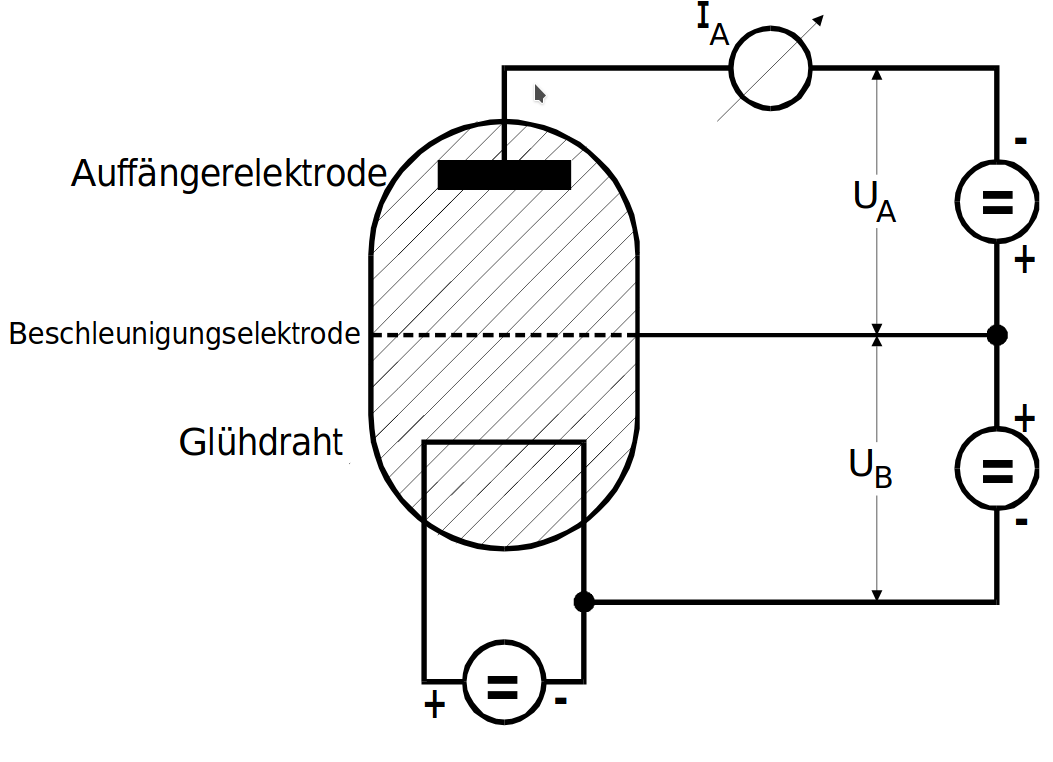
\includegraphics[width=\textwidth]{content/data/schematischeraufbau.png}
    \caption{Der schematische Aufbau zum Franck-Hertz Versuch. Bild entnommen aus der Versuchsanleitung \cite[2]{anleitung}.}
    \label{fig:schematischeraufbau}
\end{figure}

\begin{figure}
    \centering
    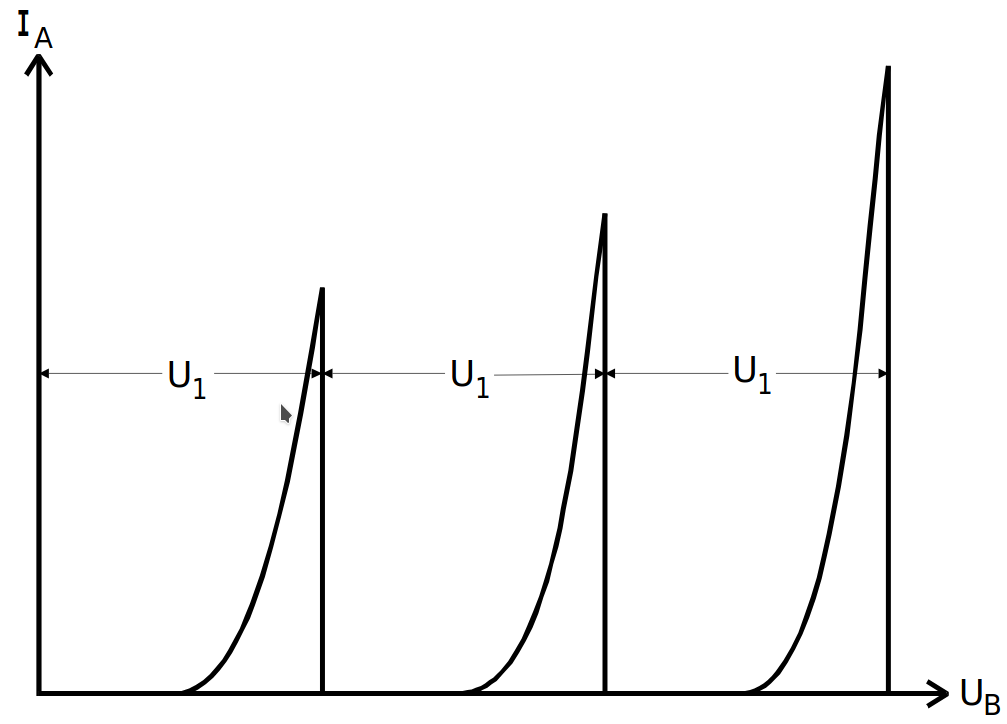
\includegraphics[width=\textwidth]{content/data/Spannungsverlauf.png}
    \caption{Der schematische Spannungsverlauf der Franck-Hertz Kurven. Bild entnommen aus der Versuchsanleitung \cite[4]{anleitung}.}
    \label{fig:spannungsverlauf}
\end{figure}

\begin{figure}
    \centering
    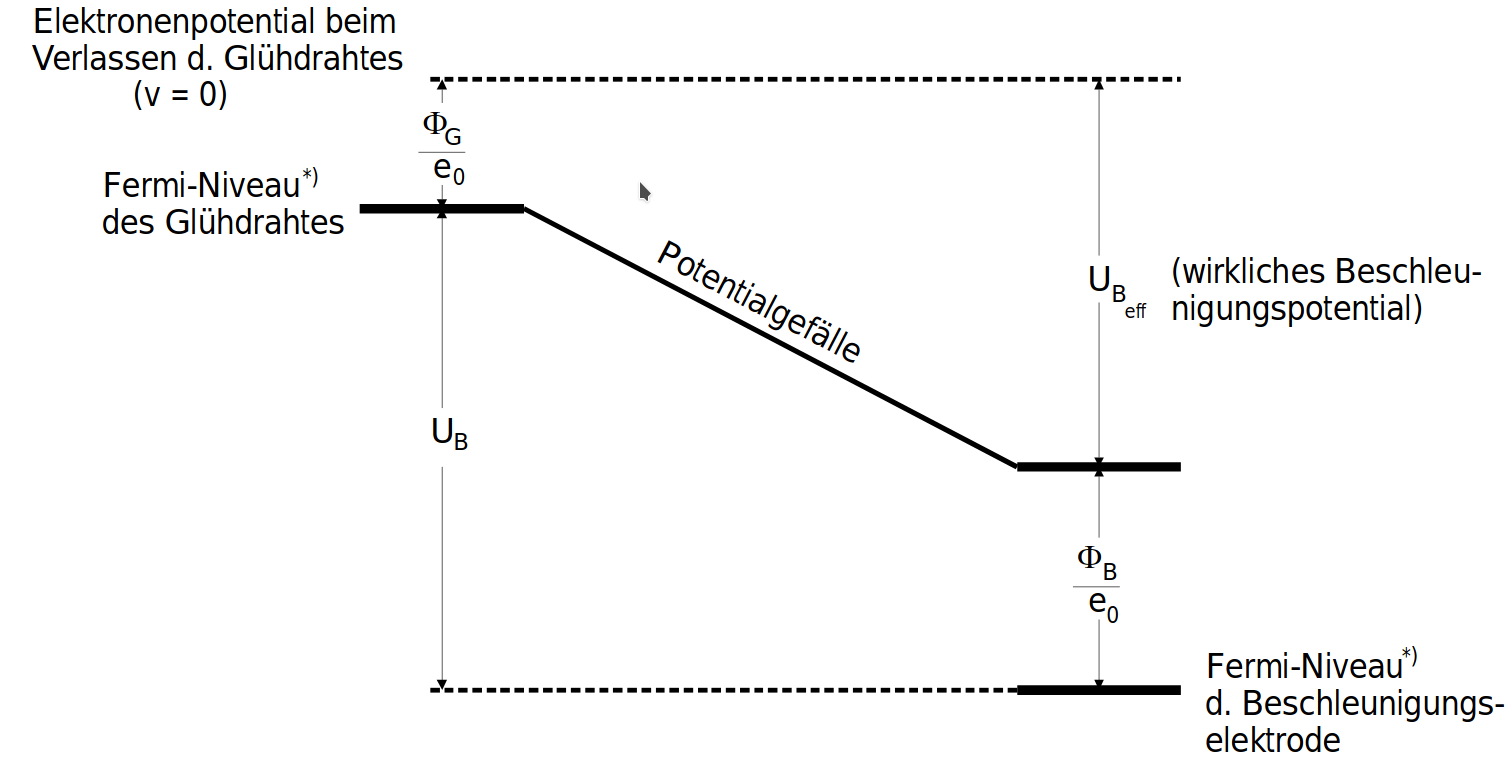
\includegraphics[width=\textwidth]{content/data/Potentialgefaelle.png}
    \caption{Das Potentiallgefälle zwischen Glühdraht und Beschleunigungselektrode. Bild entnommen aus der Versuchsanleitung \cite[5]{anleitung}.}
    \label{fig:potential}
\end{figure}

